\documentclass[]{article}
\usepackage{amsmath}\usepackage{amsfonts}
\usepackage[margin=1in,footskip=0.25in]{geometry}
\usepackage{mathtools}
\usepackage{hyperref}
\hypersetup{
    colorlinks=true,
    linkcolor=blue,
    filecolor=magenta,
    urlcolor=cyan,
}
\usepackage[final]{graphicx}
\usepackage{listings}
\usepackage{courier}
\lstset{basicstyle=\footnotesize\ttfamily,breaklines=true}
\newcommand{\indep}{\perp \!\!\! \perp}
% \usepackage{wrapfig}
\graphicspath{{.}}
% \usepackage{fancyvrb}

%%
%% Julia definition (c) 2014 Jubobs
%%
\usepackage[T1]{fontenc}
\usepackage{beramono}
\usepackage[usenames,dvipsnames]{xcolor}
\lstdefinelanguage{Julia}%
  {morekeywords={abstract,break,case,catch,const,continue,do,else,elseif,%
      end,export,false,for,function,immutable,import,importall,if,in,%
      macro,module,otherwise,quote,return,switch,true,try,type,typealias,%
      using,while},%
   sensitive=true,%
   alsoother={$},%
   morecomment=[l]\#,%
   morecomment=[n]{\#=}{=\#},%
   morestring=[s]{"}{"},%
   morestring=[m]{'}{'},%
}[keywords,comments,strings]%

\lstset{%
    language         = Julia,
    basicstyle       = \ttfamily\footnotesize
    keywordstyle     = \bfseries\color{blue},
    stringstyle      = \color{magenta},
    commentstyle     = \color{ForestGreen},
    showstringspaces = false,
}
\begin{document}
\begin{center}
    Name: Hongda Li 
    AMATH 585 WINTER 2022 HW5
\end{center}
\section*{The Code}
    The following code is the implementation for both problem 1, 2
    \lstinputlisting{hw5_script.jl}
\section*{Problem 1}
    \subsection*{Theory that goes with the code}
        \hspace{1.1em}
        Natural ordering of the element refers to the mapping of tuple of indices from the grid to the actual point in space, given as $u_{i, j} = u(ih, jh)$. Here, we use equally space point in both xy direction on the unit square: $[0, 1]\times [0, 1]$. And we use $m$ number of interior points, and including the boundary we will have $m + 2$ boundary point. 
        \par
        The implementation focuses on building up the system of matrices using the stencil defined on each point indexed grid point $(i, j)$. For each point, we convert the coordinate indices $(i, j)$ to linear indices for row and column location in the sparse matrix, the coefficient on the stencil is then added to the matrix or the RHS of the system. This is done for $(i, j) \in \{0, 1, \cdots, m\}^2$. If any of the point are laying outside, we move the coefficient to the RHS vector. 
        \par
        Alternatively, one can also use Kronecker Product to construct the structural matrice, but it will lose the elegence of on the code and less generic. Algebraically, one can handle the boundary conditions by thinking about the stencils on the boundary. I only did it for the 5 point stencil. 
        \par
        Let $\mathcal{I}(i, j) = (j - 1)m + i \quad \forall (i, j) \in [1, \cdots, m]\times[1, \cdots m]$ be a mapping from the coordinate indices of the grid point to linear index. Next, we consider partitioning the vector $u$ and $b$ the RHS vector by rows on the grid using natural ordering. 
        \begin{align*}\tag{1.1}\label{eqn:1.1}
            u &= \begin{bmatrix}
                u^{[1]} \\ u^{[2]} \\ \vdots \\ u^{[m]}
            \end{bmatrix}
            \;
            \vec{b} = \begin{bmatrix}
                b^{[1]} \\ b^{[2]} \\ \vdots \\ b^{[m]}
            \end{bmatrix}
            \;
            \vec{f} = \begin{bmatrix}
                f^{[1]} \\ f^{[2]}\\ \vdots \\ f^{[m]}
            \end{bmatrix}
            \\
            u^{[i]} &= 
            \begin{bmatrix}
                u_{1, i} \\ u_{2, i} \\ \vdots \\ u_{m, i}
            \end{bmatrix}
        \end{align*}
        
        \par
        For the bounary conditions, we consider them row by row. Consider the first row: 
        \begin{align*}\tag{1.2}\label{eqn:1.2}
            \begin{aligned}
                \vec{f}_{\mathcal{I}(i, 1)} &= 
                \frac{1}{h^2}
                \text{sum}
                \left(
                    \begin{bmatrix}
                        & u_{i, 2}& 
                        \\
                        u_{i - 1, 1} & -4u_{i, 1}& u_{i + 1, 1}
                        \\
                        & u_{i, 0}& 
                    \end{bmatrix}
                \right) \quad \forall 1 \le i \le m
                \\
                \vec{b}^{[1]} &= 
                - \frac{1}{h^2}\begin{bmatrix}
                    u_{1, 0} \\ u_{2, 0} \\ \vdots \\ u_{m, 0}
                \end{bmatrix}
                - \frac{u_{0, 1}\mathbf{e}_1^{(m)}}{h^2} 
                - \frac{u_{m + 1, 1} \mathbf{e}_{m}^{(m)}}{h^2}
                + f^{[1]}
            \end{aligned}
        \end{align*}
        Next, we consider all the rows in the middle rows: 
        \begin{align*}\tag{1.3}\label{eqn:1.3}
            \begin{aligned}
                \vec{f}_{\mathcal{I}(i, j)} &= 
                \frac{1}{h^2}
                \text{sum}
                \left(
                    \begin{bmatrix}
                        & u_{i, j + 1}& 
                        \\
                        u_{i - 1, j} & -4u_{i, j}& u_{i + 1, j}
                        \\
                        & u_{i, j - 1}& 
                    \end{bmatrix}
                \right) \quad \forall 1 \le i \le m , \; 2 \le j \le m - 1
                \\
                \vec{b}^{[j]} &= 
                - \frac{u_{0, j}\mathbf{e}_{1}^{(m)}}{h^2}
                -
                \frac{u_{m+ 1,j}\mathbf{e}_m^{(m)}}{h^2}
                + f^{[j]}
            \end{aligned}
        \end{align*}
        Finally we consider the last row on the grid point: 
        \begin{align*}\tag{1.4}\label{eqn:1.4}
            \begin{aligned}
                \vec{f}_{\mathcal{I}(i, m)} &= 
                \frac{1}{h^2}\text{sum}
                \left(
                    \begin{bmatrix}
                        & u_{i, m + 1}&  \\
                        u_{i- 1, j}& -4u_{i, m}&  u_{i + 1, j} \\
                        & u_{i, m - 1}&  
                    \end{bmatrix}
                \right)
                \quad \forall\; 1 \le i \le m
                \\
                b^{[m]} &= 
                -\frac{1}{h^2}\begin{bmatrix}
                    u_{1, m + 1} \\ u_{2, m _ 1} \\ \vdots \\ u_{m, m + 1}
                \end{bmatrix} 
                - \frac{u_{0, m}}{h^2}\mathbf{e}^{(m)}_1 
                - \frac{u_{m + 1, m}}{h^2}\mathbf{e}^{(m)}_m
                + \vec{f}^{[m]}
            \end{aligned}
        \end{align*}
        This completes the analysis for the RHS vector that includes the boundary. Take notice that a very different approach has been coded. This part is just for analysis. 
    \subsection*{$\mathcal{O}(h^2)$ Convergence Rate}
        \hspace{1.1em}
        Error computations is made by comparing solution on sparser grid point with the solution obtained on a fine grid point. I don't happen to know the solution of the PDE besides the solution expressed using the Green's function with the given density function.
        \par
        For the implementation of this part, refers to the ``Problem1()'' function. The finer grid is taken with $m = 2^{10} - 1$, and then $m$ follows the pattern of $2^{k} - 1$ so that the discretized grid-point of the sparser grids is a subset of the finer grid. This is a plot of the error measured by $L2$ norm in 2D in log log plot, referenced with $h^2$ convergence: 
        \begin{center}
            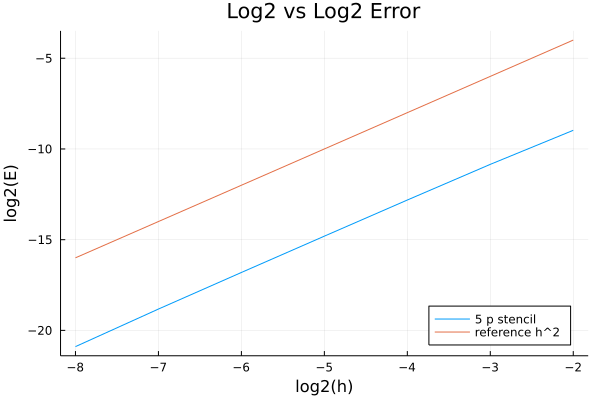
\includegraphics[width=10cm]{p1_fig.png}
        \end{center}
        Numerically, I take the slope of the adjacent points on the log log plot and take the averaging, producing an estimate of the rate of convergence for the 5 points stencil method. The esimated rate is: $1.986773401321141$. 
\section*{Problem 2}
    \hspace{1.1em}
    The same routine is run for the 9-point stencils but with a different definition of the stencil. Deferred correction is implemented by the end, right before the calculation of solution. 
    \par 
    The estimated rate of convergnece of error is $3.0268502045280115$, The error is $\mathcal{O}(n^3)$, which differs from the theory. Here is a plot of the error under log log plot: 
    \begin{center}
        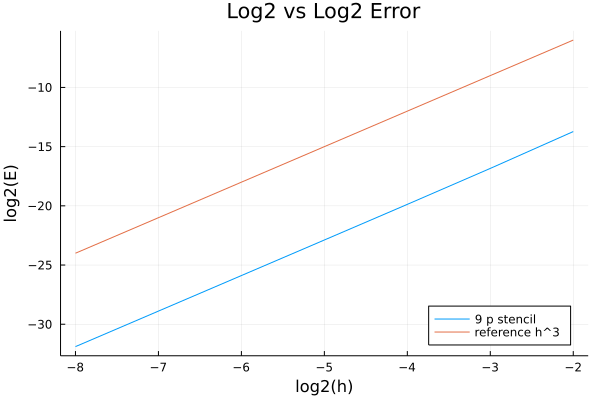
\includegraphics[width=10cm]{p2_fig.png}
    \end{center}
    Observe that this is a mismatch from what is predicted by the theory where it's stated that with deferred correction, the error should have convergence rate of $\mathcal{O}(h^4)$. 

        

\end{document}